\documentclass[11pt]{article}
\usepackage{blindtext}
\usepackage{gensymb}
\usepackage{booktabs}
\usepackage{graphicx}
\usepackage{caption}
\usepackage[a4paper, total={6.5in, 10in}]{geometry}
\begin{document}
\author{Raunak Jalan}
\title{Statistical Analysis of NIFTY50 Index}
\maketitle

\section*{Abstract}

This report is focused on applying various statistical methods on Indian Stock Market to get meaningful conclusions which will be helpful from an investor point of view or who fears to enter the stock market. We can use the data of NIFTY50 index to approximate the Indian stock market, using it's historical data from 2013 to 2022. We won't incorporate any other factors since we want only mathematical results. Other real life factor inclusion will only increase the chances of gaining money from the stock market.

\section*{The Historical Trend}

If we plot the NIFTY50 index prices v/s days passed. We get the following figure.

\begin{center}
 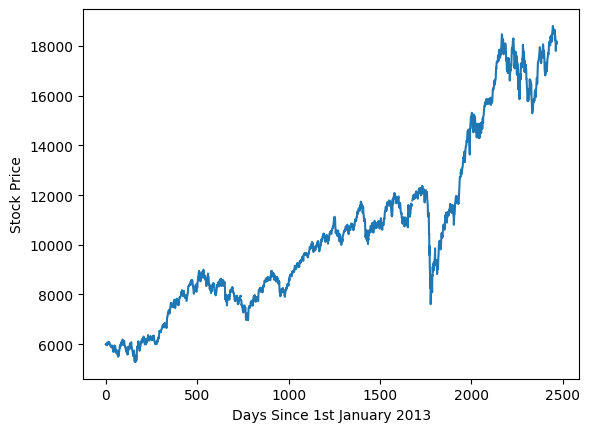
\includegraphics[scale=1.05]{prices.png}
\end{center}

\begin{flushleft}
\textbf{Conclusion based on the above analysis}: Stock prices may change in a highly volatile manner within a short period of time but for longer period of time, they are going to make you money, ofcourse if the macroeconomic conditions are normal.
\end{flushleft}
Holding index stocks for a longer period of time may be a good strategy to invest your money.
\newpage

\section*{Modelling The Stock Market}
\vspace{7mm}

Due to the extremely volatile nature of the stock market, it is really difficult to model the stock market, or more specifically predict the stock market prices or returns.\
To easen out the calculations, we will consider the logarithms of the daily returns to do the modelling.\\

After doing so, we get the following plot:

\begin{center}
 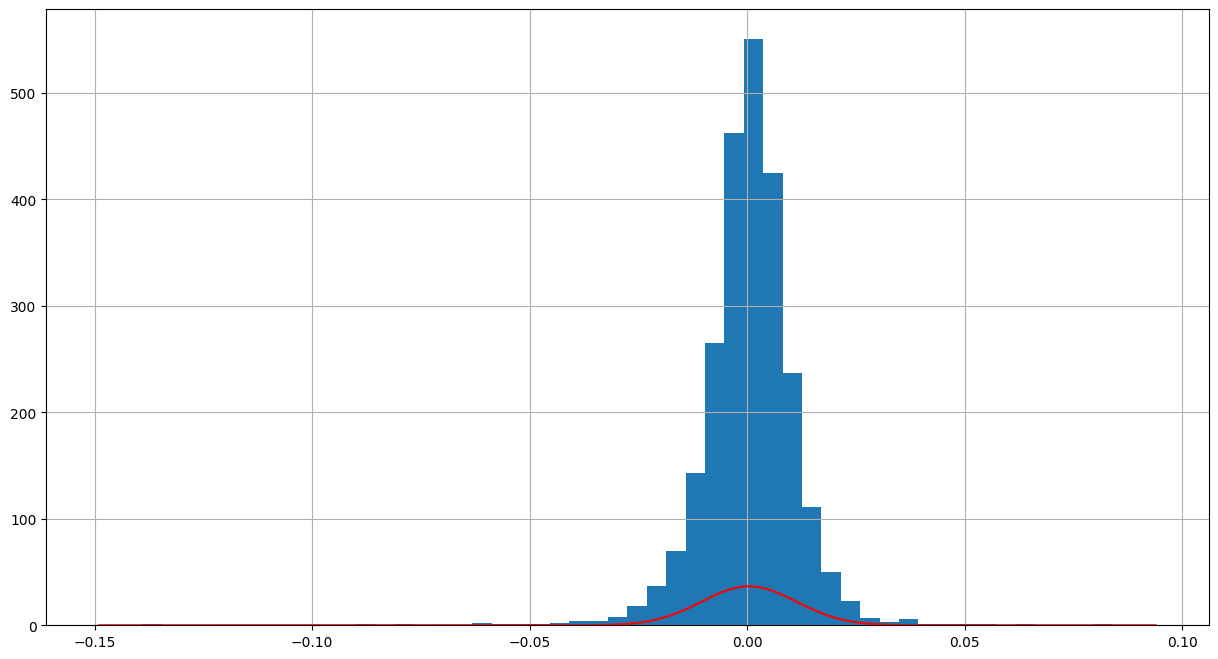
\includegraphics[scale=0.53]{normal.png}
\end{center}
\vspace{5mm}
We can see that the log of daily returns is approximately normally distributed, so we can model the stock market returns using normal distribution. \\

We will find the mean and stand deviation of the log of daily returns for further analysis.
\\

\section*{Calculating Risk In Daily Returns}

Imagine you are not a long term investor but an intraday trader who buys shares exactly when the market opens and sells all the shares exactly when the market closes. You want to know the probability if you are more likely to make money or lose money if you follow this strategy.\\

To determine the probability of getting negative returns, we will calculate the area under the normal distribution centered at mean and stand deviation we got earlier, till the 0 mark.\\

Doing so, we get the probability to be 48.34\% which is slightly less than 50\%, which means there is almost equal chances of gaining and losing money with a very slight bias towards gaining money.\

\vspace{4mm}
\raggedright \textbf{Conclusion based on the above analysis:} The daily returns can be modelled like a coin toss, with equal probability of gaining or losing money.
\newpage

\section*{Estimating Volatility Of The Index} 
\vspace{8mm}
If we again use the cumulative distribution function to determine the probabilities of losing a specific \% of the current price in a day, we get the following values:

\begin{table}[ht]
  \centering
  \caption{Gain/Loss and Probability}
  \begin{tabular}{cc}
    \toprule
    \textbf{Loss \%} & \textbf{Probability (\%)} \\
    \midrule
    -10\% & 1.5820655994303313e-18 \% \\
    -5\% & 0.00018 \% \\
    -2.5\% & 0.97 \% \\
    -1\% & 16.88 \% \\
    0\% & 48.34\% \\
    \bottomrule
  \end{tabular}
\end{table}

We can see, the probability of having significant movements in the daily price decreases as the change in prices increases. Depending on the personal risk taking capacity one can chose what amount to trade.\\
\vspace{2.5mm}
Similarly, for long term investments, say 1 year, we get the following values:


\begin{table}[ht]
  \centering
  \caption{Gain/Loss and Probability}
  \begin{tabular}{cc}
    \toprule
    \textbf{Gain/Loss \%} & \textbf{Probability (\%)} \\
    \midrule
    -10\% & 10.16\% \\
    -5\% & 15.09\% \\
    -2.5\% & 18.08\% \\
    -1\% & 20.03\% \\
    0\% & 21.4\% \\
    +1\% & 77.16\% \\
    +2.5\% & 74.92\% \\
    +5\% & 70.95\% \\
    +10\% & 62.25\% \\
    \bottomrule
  \end{tabular}
\end{table}
\vspace{2mm}

What if we increase the duration to 1000 days? We get the following data:

\begin{table}[ht]
  \centering
  \caption{Gain/Loss and Probability}
  \begin{tabular}{cc}
    \toprule
    \textbf{Gain/Loss \%} & \textbf{Probability (\%)} \\
    \midrule
    -10\% & 5.46\% \\
    -5\% & 7.26\% \\
    -2.5\% & 8.32\% \\
    -1\% & 9\% \\
    0\% & 9.48\% \\
    +1\% & 90.01\% \\
    +2.5\% & 89.22\% \\
    +5\% & 87.82\% \\
    +10\% & 84.64\% \\
    +20\% & 76.76\% \\
    +30\% & 67.04\% \\
    \bottomrule
  \end{tabular}
\end{table}

\vspace{10mm}
\textbf{Conclusion Based On The Above Analysis:} 
\begin{itemize}
\item There is some risk associated with long term investing, but the risk decreases as we move from 365 days to 1000 days, hence more the chance of getting more returns from the market.
\item The probability of losing the same amount of money is very less than making the same amount of money in 1 year, which implies the positive side of long term investing.
\end{itemize}

\section*{Value At Risk}
\vspace{5mm}
Value at Risk or VaR tells us how much we could lose over a specific holding period with a defined probability.\\
\vspace{2mm}
We can calculate VaR using the Percent Point Function (ppf).\\

\begin{verbatim}
var = norm.ppf(0.05, mu, sigma) = -1.7 %
\end{verbatim}
\vspace{1mm}

It means there is a 5\% chance for daily returns to be worse than -1.7\%. Similarly, we can determine VaR for different probability values.

\section*{Average Returns Using Confidence Intervals}
\vspace{5mm}
Confidence intervals are a statistical concept used to estimate the range within which a population parameter, such as the mean or proportion, is likely to fall. It provides a range of values rather than a single point estimate and is associated with a certain level of confidence.\\

We shall find out the 95\% confidence intervals for daily returns:
\begin{verbatim}
sample_size = data['LogReturn'].shape[0] # n data points
sample_mean = data['LogReturn'].mean() # mean of the population
sample_std = data['LogReturn'].std(ddof=1) / sample_size**0.5
# standard deviation of the population divided by sqrt(n) = standard deviation of sample.

# left and right quantile # 90% confidence interval means, 1-a = 0.9 (area % as fraction)
# which gives a = 0.1, so a/2 is 0.05 and 1-a/2 is 0.95

z_left = norm.ppf(0.05) # left quantile score
z_right = norm.ppf(0.95) # right quantile score
z = z_right
# also, z = abs(z_left)

# upper and lower bounds
interval_left = sample_mean - sample_std*z
interval_right = sample_mean + sample_std*z
\end{verbatim}

Which leaves us with 90\% confidence interval for daily average returns being in the range (0.009, 0.08)\% which means there is slight chance of getting positive returns (Which we earlier mentioned).
\newpage
\section*{Final Conclusion \& Key Points}
\vspace{1cm}
The statistical analysis of the NIFTY50 Index provides valuable insights for investors seeking a data-driven perspective on the Indian stock market. Here's a summary of key findings from the methods employed:

\subsection*{Historical Trend Analysis:}

\begin{itemize}
  \item Long-term investment in NIFTY50 index stocks appears to be a viable strategy, given the observed trend over time.
  \item The conclusion suggests that, despite short-term volatility, there is potential for positive returns over an extended period under normal macroeconomic conditions.
\end{itemize}

\subsection*{Modeling The Stock Market:}

\begin{itemize}
  \item The decision to model daily returns using the logarithm facilitates calculations and analysis, revealing a distribution that approximates normality.
\end{itemize}

\subsection*{Risk in Daily Returns:}

\begin{itemize}
  \item The analogy of daily returns to a coin toss, with nearly equal probabilities of gaining or losing money, implies a certain unpredictability in short-term outcomes.
\end{itemize}

\subsection*{Estimating Volatility:}

\begin{itemize}
  \item The analysis of probabilities for different gain/loss scenarios over varying time horizons provides investors with insights into potential market movements.
  \item Longer-term investments show a decreasing risk profile, suggesting a positive correlation between investment duration and the probability of positive returns.
\end{itemize}

\subsection*{Value at Risk (VaR):}

\begin{itemize}
  \item The calculation of VaR at a 5\% probability level indicates the potential downside risk, allowing investors to assess the potential loss over a specific holding period.
\end{itemize}

\subsection*{Average Returns Using Confidence Intervals:}

\begin{itemize}
  \item The 90\% confidence interval for daily average returns provides a range (0.009\%, 0.08\%) where the true mean is likely to fall, aiding investors in understanding the potential variation in daily returns.
\end{itemize}

In summary, the analysis suggests that while short-term fluctuations may resemble a coin toss, long-term investment in the NIFTY50 Index carries a higher probability of positive returns. Understanding volatility, assessing risk through VaR, and considering confidence intervals for average returns contribute to a more informed approach to investment decisions. This statistical exploration serves as a valuable tool for investors navigating the dynamic landscape of the Indian stock market.

\end{document}